\section{Результаты}
\label{sec:Results} \index{Results}

\subsection{Словари}

\noindent\hspace{0.6cm}В первую очередь интересно рассмотреть распределение слов наиболее часто подверженных атаке для обоих датасетов и для всех методов извлечения важности. По вертикали расположены слова, по гризонтали - частота:

\begin{itemize}
    \item Для датасета с отзывами на банки \textbf{SentiRuEval-2016-banks}
\end{itemize}

\begin{figure}[H]
\centering
\begin{minipage}[b]{0.49\textwidth}
\centering
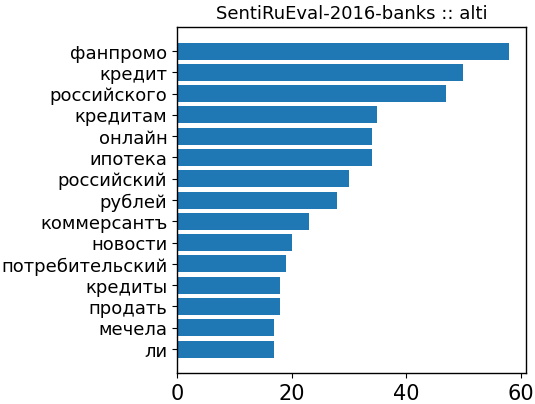
\includegraphics[width=\textwidth]{pictures/examples_banks/dict1.png} % Замените image1 на имя файла первой картинки
\caption{ALTI}
\end{minipage}
\hfill
\begin{minipage}[b]{0.49\textwidth}
\centering
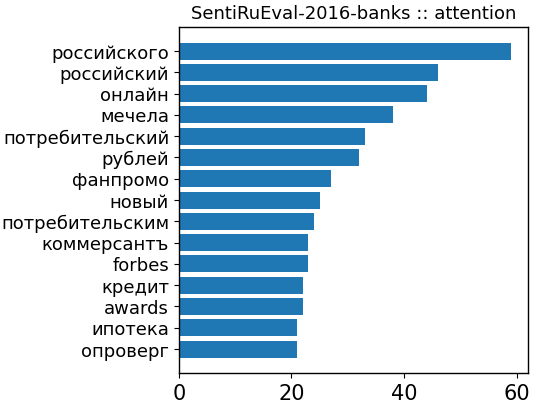
\includegraphics[width=\textwidth]{pictures/examples_banks/dict2.png} % Замените image2 на имя файла второй картинки
\caption{Attention}
\end{minipage}
\end{figure}

\begin{figure}[H]
\centering
\begin{minipage}[b]{0.49\textwidth}
\centering
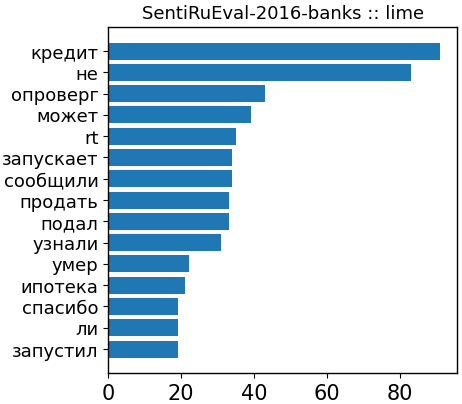
\includegraphics[width=\textwidth]{pictures/examples_banks/dict3.png} % Замените image1 на имя файла первой картинки
\caption{LIME}
\end{minipage}
\hfill
\begin{minipage}[b]{0.49\textwidth}
\centering
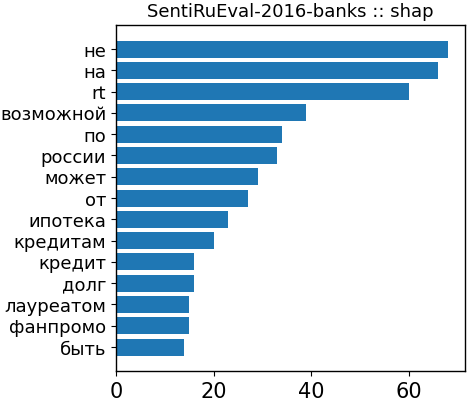
\includegraphics[width=\textwidth]{pictures/examples_banks/dict4.png} % Замените image2 на имя файла второй картинки
\caption{SHAP}
\end{minipage}
\end{figure}

\begin{figure}[H]
\centering
\begin{minipage}[b]{0.49\textwidth}
\centering
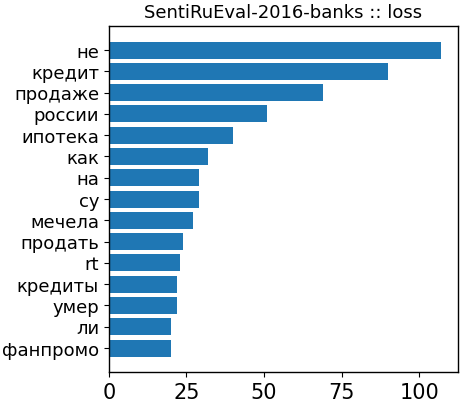
\includegraphics[width=\textwidth]{pictures/examples_banks/dict5.png} % Замените image1 на имя файла первой картинки
\caption{Loss}
\end{minipage}
\hfill
\begin{minipage}[b]{0.49\textwidth}
\centering
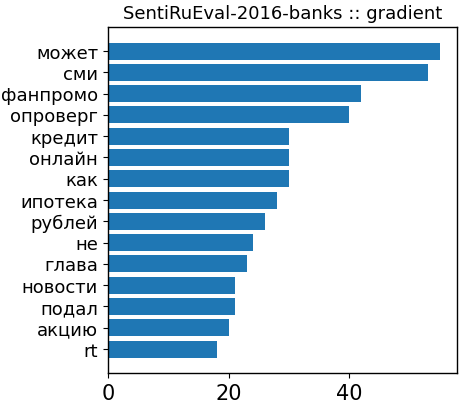
\includegraphics[width=\textwidth]{pictures/examples_banks/dict6.png} % Замените image2 на имя файла второй картинки
\caption{Gradient}
\end{minipage}
\end{figure}

\noindent\hspace{0.6cm}Исходя из вида полученных словарей наиболее часто выделяемых слов различных методами интерпретации можно сделать вывод, что почти все подходы в основном выделяют слова, связанные с банковской тематикой. Тем не менее некоторые методы, например SHAP, очень часто выделяют слова слабо относящиеся к данной тематике (как видно из рисунка, например, это частица не и прилагательное возможной). Данная корреляция может быть связана с тем, что атакуемая модель была дообучена не на самое высокое качество на используемом датасете.

\newpage
\begin{itemize}
\item Для датасета с отзывами на компании сотовой связи \textbf{SentiRuEval-2016-telecoms}

\begin{figure}[H]
\centering
\begin{minipage}[b]{0.49\textwidth}
\centering
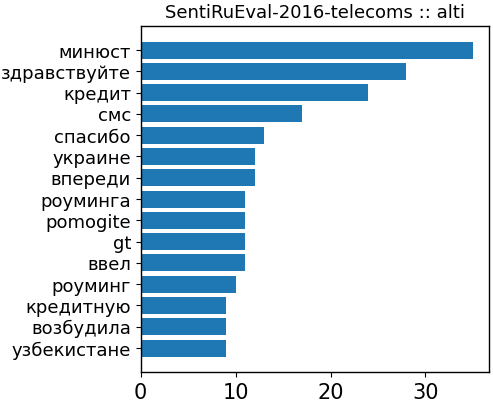
\includegraphics[width=\textwidth]{pictures/examples_telecoms/dct1.png} % Замените image1 на имя файла первой картинки
\caption{ALTI}
\end{minipage}
\hfill
\begin{minipage}[b]{0.49\textwidth}
\centering
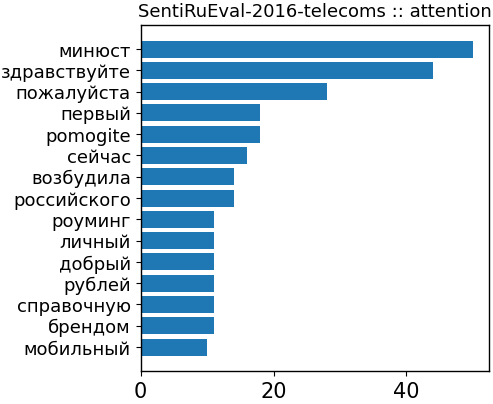
\includegraphics[width=\textwidth]{pictures/examples_telecoms/dct2.png} % Замените image2 на имя файла второй картинки
\caption{Attention}
\end{minipage}
\end{figure}

\begin{figure}[H]
\centering
\begin{minipage}[b]{0.49\textwidth}
\centering
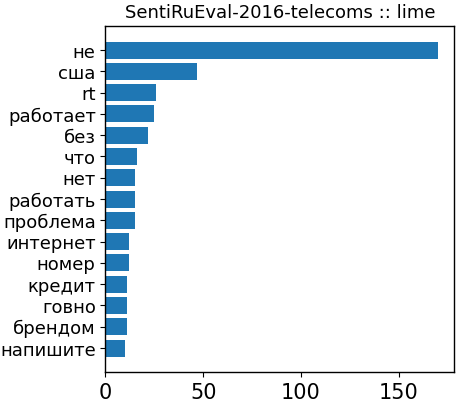
\includegraphics[width=\textwidth]{pictures/examples_telecoms/dct3.png} % Замените image1 на имя файла первой картинки
\caption{LIME}
\end{minipage}
\hfill
\begin{minipage}[b]{0.49\textwidth}
\centering
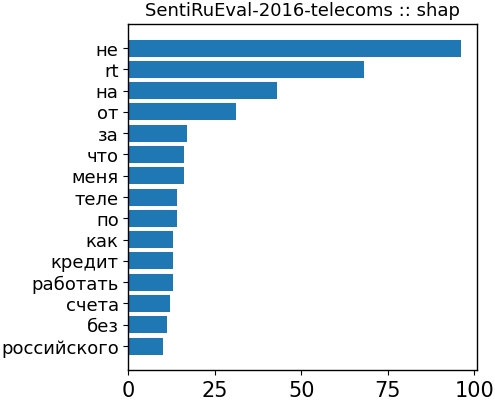
\includegraphics[width=\textwidth]{pictures/examples_telecoms/dct4.png} % Замените image2 на имя файла второй картинки
\caption{SHAP}
\end{minipage}
\end{figure}

\begin{figure}[H]
\centering
\begin{minipage}[b]{0.49\textwidth}
\centering
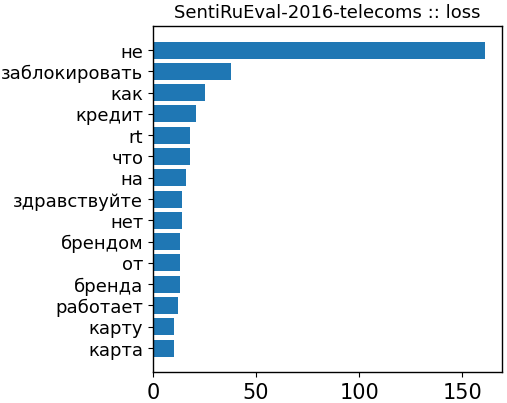
\includegraphics[width=\textwidth]{pictures/examples_telecoms/dct5.png} % Замените image1 на имя файла первой картинки
\caption{Loss}
\end{minipage}
\hfill
\begin{minipage}[b]{0.49\textwidth}
\centering
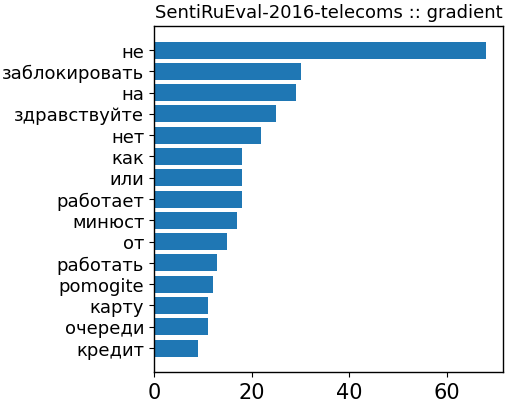
\includegraphics[width=\textwidth]{pictures/examples_telecoms/dct6.png} % Замените image2 на имя файла второй картинки
\caption{Gradient}
\end{minipage}
\end{figure}

\end{itemize}

\noindent\hspace{0.6cm}Исходя из вида полученных словарей наиболее часто выделяемых слов различных методами интерпретации можно сделать вывод, что большинство подходов в основном выделяют слова, которые мало связаны с тематикой телекомпаний. Тем не менее некоторые методы, например ALTI, иногда выделяют слова относящиеся к данной тематике (например, слова роуминг или смс, как видно из рисунка). Данная корреляция как и в случае с предыдущим датасетом может быть связана с тем, что атакуемая модель была дообучена не на самое высокое качество на используемых данных.

\newpage
\subsection{Время работы}

\noindent\hspace{0.6cm}Ниже указано время работы каждого метода в секундах. Стоит отметить, что некоторые методы можно оптимизировать по скорости работы, например, \textbf{SHAP} и \textbf{LIME} за счет подбора гиперпараметров: для SHAP - количество различных маргинальных контрибуций, для LIME - объем генерируемой выборки и параметры обучаемой Logistic Regression, - однако в таком случае это может сказаться на итоговом качестве сгененрированных состязательных примеров

\begin{table}[h]
  \centering
  {\renewcommand{\arraystretch}{1.5}
  \caption{Среднее время работы методов оптимизации}
  {\fontsize{11pt}{10pt}\selectfont
  \begin{tabularx}{\textwidth}{|l|X|X|X|X|X|X|}
    \hline
     & lime         & shap         & loss         & gradient         & alti      & attention  \\
    \hline
     время работы      & 0.23 & 0.08 & 0.04 & 0.046 & 0.11 & 0.007\\
    \hline
    \end{tabularx}
    }
    }
\end{table}

\subsection{Итоговые показатели}

\noindent\hspace{0.6cm}Ниже представленые таблицы для каждого рассматривамого датасета и для 1-2 искаженных слов, где в строках расположены исследуемые методы оптимизации, а в столбцах - способы генерации состязательных примеров. На пересечении находятся 3 значения в слeдующем формате \textbf{ASR/BERT\_USE/DAN\_USE}. Жирным шрифтом выделены лучшие показатели \textbf{ASR} для каждого столбца. Под \textbf{ins\_char} подразумевается вставка символа, \textbf{del\_char} - удаление символа, \textbf{sub\_char} - замена символа случайным ближайшим на клавиатуре, \textbf{sub\_word} - замена слова синонимом, \textbf{del\_word} - удаление наиболее важного слова из текста. В каждой колонке для удобства восприятия добавлена приписка \textbf{AR/BU/DU} (сокращение от \textbf{ASR/BERT\_USE/DAN\_USE}). Также в самой последней строчке у всех таблиц приведены усредненные значения по каждому столбцу.

\begin{table}[H]
  \centering
  \caption{SentiRuEval-2016-banks :: искажение 1 слова}
  {\renewcommand{\arraystretch}{1.5}
  {\fontsize{9pt}{10pt}\selectfont
  \begin{tabularx}{\textwidth}{|l|X|X|X|X|X|}
    \hline
     method    & del\_word         & ins\_char         & del\_char         & sub\_char         & sub\_word         \\
    \hline
     & AR/BU/DU & AR/BU/DU  & AR/BU/DU  & AR/BU/DU  & AR/BU/DU \\
    \hline
     alti      & 15/0.93/0.85 & 12/0.95/0.84 & 10/0.96/0.84 & 12/0.95/0.84 & 15/0.9/0.85 \\
    \hline
     attention & 12/0.95/0.85 & 9/0.97/0.84  & 8/0.97/0.84  & 8/0.97/0.84  & 12/0.94/0.85 \\
    \hline
     gradient  & 16/0.95/0.85 & 11/0.96/0.84 & 11/0.97/0.84 & 12/0.96/0.84 & 15/0.94/0.83 \\
    \hline
     lime      & \textbf{22}/0.95/0.84 & 13/0.96/0.84 & \textbf{13}/0.96/0.84 & \textbf{15}/0.96/0.84 & 15/0.94/0.83 \\
    \hline
     shap      & 11/0.96/0.84 & 11/0.96/0.83 & 9/0.97/0.83  & 11/0.96/0.83 & 12/0.95/0.84 \\
    \hline
     loss      & 20/0.95/0.84 & \textbf{14}/0.96/0.84 & \textbf{13}/0.96/0.84 & 14/0.96/0.84 & \textbf{17}/0.94/0.84 \\
    \hline
     random    & 8/0.97/0.86 & 7/0.96/0.87  & 7/0.97/0.86  & 6/0.97/0.87  & 9/0.95/0.86 \\
    \hline
     \textbf{avg\_value} & \cellcolor{gray!25} & 11/0.96/0.843 & 10.1/0.966/0.841 & 11.1/0.961/0.843 & \textbf{13.6}/0.937/0.843 \\
    \hline
    \end{tabularx}
    }
    }
\end{table}

\begin{table}[H]
  \centering
  \caption{SentiRuEval-2016-telecoms :: искажение 1 слова}
  {\renewcommand{\arraystretch}{1.5}
  {\fontsize{9pt}{10pt}\selectfont
  \begin{tabularx}{\textwidth}{|l|X|X|X|X|X|}
    \hline
     method    & del\_word         & ins\_char         & del\_char         & sub\_char         & sub\_word         \\
    \hline
     & AR/BU/DU & AR/BU/DU  & AR/BU/DU  & AR/BU/DU  & AR/BU/DU \\
    \hline
     alti      & 13/0.94/0.9 & 10/0.96/0.89 & 10/0.96/0.89 & 11/0.95/0.89 & 15/0.91/0.89 \\
    \hline
     attention & 11/0.95/0.9 & 8/0.97/0.89  & 8/0.97/0.89  & 8/0.97/0.89  & 11/0.94/0.89 \\
    \hline
     gradient  & 14/0.96/0.89 & 11/0.97/0.89 & 10/0.97/0.89 & 11/0.97/0.89 & 14/0.95/0.89 \\
    \hline
     lime      & \textbf{21}/0.96/0.88 & \textbf{13}/0.97/0.87 & \textbf{13}/0.97/0.87 & \textbf{14}/0.96/0.87 & 15/0.95/0.89 \\
    \hline
     shap      & 10/0.97/0.89 & 8/0.97/0.88  & 7/0.97/0.88  & 9/0.97/0.88  & 10/0.95/0.87 \\
    \hline
     loss      & \textbf{21}/0.96/0.89 & \textbf{13}/0.96/0.88 & 11/0.97/0.88 & \textbf{14}/0.96/0.88 & \textbf{16}/0.95/0.88 \\
    \hline
     random    & 8/0.97/0.91 & 6/0.98/0.9  & 5/0.97/0.91  & 5/0.96/0.91  & 8/0.96/0.9 \\
    \hline
     \textbf{avg\_value} & \cellcolor{gray!25} & 9.9/0.969/0.886 & 9.1/0.969/0.887 & 10.3/0.963/0.887 & \textbf{12.7}/0.944/0.887 \\
    \hline
    \end{tabularx}
    }
    }
\end{table}

\begin{table}[H]
  \centering
  \caption{SentiRuEval-2016-banks :: искажение 2 слов}
  {\renewcommand{\arraystretch}{1.5}
  {\fontsize{9pt}{10pt}\selectfont
  \begin{tabularx}{\textwidth}{|l|X|X|X|X|X|}
    \hline
     method    & del\_word         & ins\_char         & del\_char         & sub\_char         & sub\_word         \\
    \hline
     & AR/BU/DU & AR/BU/DU  & AR/BU/DU  & AR/BU/DU  & AR/BU/DU \\
    \hline
     alti      & 19/0.88/0.8 & 18/0.92/0.81 & 14/0.92/0.81 & 17/0.91/0.81 & 20/0.85/0.81 \\
    \hline
     attention & 18/0.9/0.8 & 14/0.93/0.8  & 12/0.94/0.8  & 16/0.93/0.8  & 18/0.88/0.81 \\
    \hline
     gradient  & 22/0.91/0.8 & 18/0.93/0.8  & 16/0.94/0.8  & 18/0.93/0.8  & 20/0.9/0.8 \\
    \hline
     lime      & \textbf{30}/0.91/0.78 & \textbf{20}/0.92/0.78 & \textbf{19}/0.93/0.78 & \textbf{21}/0.92/0.78 & \textbf{21}/0.89/0.79 \\
    \hline
     shap      & 17/0.93/0.79 & 15/0.93/0.79 & 14/0.94/0.79 & 16/0.93/0.79 & 17/0.9/0.8 \\
    \hline
     loss      & 27/0.92/0.79 & 19/0.93/0.79 & 18/0.93/0.79 & 20/0.92/0.79 & \textbf{21}/0.89/0.8 \\
    \hline
     random    & 14/0.93/0.82 & 12/0.94/0.82 & 12/0.94/0.83 & 12/0.94/0.83 & 15/0.9/0.83 \\
    \hline
     \textbf{avg\_value} & \cellcolor{gray!25} & 16.6/0.929/0.798 & 15/0.934/0.8 & 17.1/0.926/0.8 & \textbf{18.8}/0.887/0.806 \\
    \hline
    \end{tabularx}
    }
    }
\end{table}

\begin{table}[H]
  \centering
  \caption{SentiRuEval-2016-telecoms :: искажение 2 слов}
  {\renewcommand{\arraystretch}{1.5}
  {\fontsize{9pt}{10pt}\selectfont
  \begin{tabularx}{\textwidth}{|l|X|X|X|X|X|}
    \hline
     method    & del\_word  &        ins\_char         & del\_char         & sub\_char         & sub\_word   \\
    \hline
     & AR/BU/DU & AR/BU/DU  & AR/BU/DU  & AR/BU/DU  & AR/BU/DU \\
    \hline
     alti      & 19/0.89/0.87 & 15/0.92/0.86 & 15/0.93/0.86 & 16/0.92/0.86 & 19/0.86/0.86 \\
    \hline
     attention & 17/0.91/0.86 & 13/0.94/0.86 & 12/0.94/0.86 & 13/0.94/0.86 & 16/0.89/0.86 \\
    \hline
     gradient  & 20/0.92/0.86 & 15/0.94/0.85 & 15/0.94/0.85 & 16/0.94/0.85 & \textbf{20}/0.91/0.84 \\
    \hline
     lime      & \textbf{29}/0.92/0.83 & \textbf{18}/0.93/0.83 & \textbf{18}/0.94/0.83 & 19/0.93/0.84 & \textbf{20}/0.91/0.84 \\
    \hline
     shap      & 14/0.94/0.85 & 13/0.94/0.84 & 12/0.95/0.84 & 14/0.94/0.84 & 16/0.91/0.85 \\
    \hline
     loss      & \textbf{29}/0.92/0.85 & \textbf{18}/0.93/0.84 & 17/0.94/0.84 & \textbf{20}/0.93/0.85 & 19/0.91/0.85 \\
    \hline
     random    & 11/0.94/0.88 & 10/0.95/0.88   & 9/0.95/0.87   & 9/0.94/0.88  & 13/0.92/0.87 \\
    \hline
     \textbf{avg\_value} & \cellcolor{gray!25} & 14.6/0.936/0.851 & 14/0.941/0.85 & 15.3/0.934/0.854 & \textbf{17.6}/0.901/0.853 \\
    \hline
    \end{tabularx}
    }
    }
\end{table}

\noindent\hspace{0.6cm}Исходя из полученных выше таблиц, можно сделать вывод, что, с одной стороны, в большинстве своем именно оптимизация генерации методом \textbf{LIME} приводила к наилучшим показателям метрики \textbf{ASR}. С другой стороны, почти все методы оптимизации имеют схожее значение метрик BERT\_USE и DAN\_USE, посчитанные для контроля качества в условиях заданных изначальных ограничений. Также видно, что в среднем метод генерации, суть которого заключается в замене наиболее важных слов синонимами, дает наилучший показатель метрики \textbf{ASR}, когда как для других способов (ins\_char, del\_char, sub\_char) показатель метрики ASR ниже при одинаковых значениях DAN\_USE.

\noindent\hspace{0.6cm}Также аналогично для датасета \textbf{SentiRuEval-2016-banks} было рассмотрено влияние выбора части слова, где портить символы, на итоговое качество состязательных примеров. Под \textbf{fst} подразумевается первая половина слова, \textbf{snd} - вторая половина слова, \textbf{ins} - вставка символа, \textbf{del} - удаление символа, \textbf{sub} - замена символа случайным ближайшим на клавиатуре. Результаты представлены ниже:

\begin{table}[H]
  \centering
  \begin{minipage}[t]{0.49\textwidth} % Первая таблица
    \centering
    \caption{Вставка символа в 1 слово}
    {\fontsize{9pt}{15pt}\selectfont
    \begin{tabularx}{\textwidth}{|l|X|X|}
        \hline
         method    & ins\_fst          & ins\_snd          \\
        \hline
         & AR/BU/DU & AR/BU/DU  \\
        \hline
         alti      & 12/0.95/0.84 & 12/0.95/0.84 \\
        \hline
         attention & 9/0.97/0.84  & 9/0.97/0.84  \\
        \hline
         gradient  & 11/0.96/0.84 & 11/0.96/0.84 \\
        \hline
         lime      & 13/0.96/0.84 & 13/0.96/0.84 \\
        \hline
         loss      & 14/0.96/0.84 & 14/0.96/0.84 \\
        \hline
         shap      & 11/0.96/0.83 & 11/0.96/0.83 \\
        \hline
         \textbf{avg\_value} & 11.7/0.96/0.838 & 11.7/0.96/0.838 \\
        \hline
    \end{tabularx}
    }
  \end{minipage}
  \hfill % Добавляем горизонтальный отступ между таблицами
  \begin{minipage}[t]{0.49\textwidth} % Вторая таблица
    \centering
    \caption{Вставка символа в 2 слова}
    {\fontsize{9pt}{15pt}\selectfont
    \begin{tabularx}{\textwidth}{|l|X|X|}
        \hline
         method    & ins\_fst          & ins\_snd          \\
        \hline
         & AR/BU/DU & AR/BU/DU  \\
        \hline
         alti      & 19/0.92/0.81 & 18/0.92/0.81 \\
        \hline
         attention & 14/0.93/0.8  & 14/0.93/0.8  \\
        \hline
         gradient  & 18/0.93/0.8  & 19/0.93/0.8  \\
        \hline
         lime      & 20/0.92/0.78 & 20/0.92/0.78 \\
        \hline
         loss      & 19/0.93/0.79 & 19/0.93/0.79 \\
        \hline
         shap      & 15/0.92/0.79 & 15/0.93/0.79 \\
        \hline
         \textbf{avg\_value} & 17.5/\textbf{0.925}/0.795 & 17.5/\textbf{0.927}/0.795 \\
        \hline
    \end{tabularx}
    }
  \end{minipage}
\end{table}

\begin{table}[H]
  \centering
  \begin{minipage}[t]{0.49\textwidth} % Первая таблица
    \centering
    \caption{Удалание символа в 1 слове}
    {\fontsize{8pt}{15pt}\selectfont
    \begin{tabularx}{\textwidth}{|l|X|X|}
        \hline
         method            & del\_fst          & del\_snd          \\
        \hline
         & AR/BU/DU & AR/BU/DU  \\
        \hline
         alti      & 10/0.96/0.84 & 10/0.95/0.84 \\
        \hline
         attention & 8/0.97/0.84  & 8/0.97/0.84  \\
        \hline
         gradient  & 11/0.97/0.84 & 11/0.97/0.85 \\
        \hline
         lime      & 13/0.96/0.84 & 14/0.96/0.84 \\
        \hline
         loss      & 13/0.96/0.84 & 13/0.96/0.84 \\
        \hline
         shap      & 9/0.97/0.83  & 9/0.97/0.83  \\
        \hline
         \textbf{avg\_value} & \textbf{10.7}/\textbf{0.965}/\textbf{0.838} & \textbf{10.8}/\textbf{0.963}/\textbf{0.84} \\
        \hline
    \end{tabularx}
    }
  \end{minipage}
  \hfill % Добавляем горизонтальный отступ между таблицами
  \begin{minipage}[t]{0.49\textwidth} % Вторая таблица
    \centering
    \caption{Удаление символа в 2 словах}
    {\fontsize{8pt}{15pt}\selectfont
    \begin{tabularx}{\textwidth}{|l|X|X|}
        \hline
         method            & del\_fst          & del\_snd          \\
        \hline
         & AR/BU/DU & AR/BU/DU  \\
        \hline
         alti      & 14/0.92/0.81 & 14/0.92/0.81 \\
        \hline
         attention & 12/0.94/0.8  & 12/0.94/0.8  \\
        \hline
         gradient  & 16/0.94/0.8  & 16/0.94/0.8  \\
        \hline
         lime      & 19/0.93/0.78 & 19/0.93/0.78 \\
        \hline
         loss      & 18/0.93/0.8 & 18/0.93/0.79 \\
        \hline
         shap      & 15/0.94/0.79 & 14/0.94/0.79 \\
        \hline
         \textbf{avg\_value} & \textbf{15.7}/0.933/\textbf{0.797} & \textbf{15.5}/0.933/\textbf{0.795} \\
        \hline
    \end{tabularx}
    }
  \end{minipage}
\end{table}

\begin{table}[H]
  \centering
  \begin{minipage}[t]{0.49\textwidth} % Первая таблица
    \centering
    \caption{Замена символа в 1 слове}
    {\fontsize{9pt}{15pt}\selectfont
    \begin{tabularx}{\textwidth}{|l|X|X|}
        \hline
         method            & sub\_fst          & sub\_snd          \\
        \hline
         & AR/BU/DU & AR/BU/DU  \\
        \hline
         alti      & 12/0.95/0.84 & 12/0.95/0.84 \\
        \hline
         attention & 9/0.97/0.84  & 8/0.97/0.84  \\
        \hline
         gradient  & 12/0.96/0.84 & 13/0.96/0.84 \\
        \hline
         lime      & 15/0.96/0.84 & 15/0.96/0.84 \\
        \hline
         loss      & 14/0.96/0.85 & 14/0.96/0.84 \\
        \hline
         shap      & 11/0.96/0.83 & 11/0.96/0.83 \\
        \hline
         \textbf{avg\_value} & 12.2/0.96/\textbf{0.84} & 12.2/0.96/\textbf{0.838} \\
        \hline
    \end{tabularx}
    }
  \end{minipage}
  \hfill % Добавляем горизонтальный отступ между таблицами
  \begin{minipage}[t]{0.49\textwidth} % Вторая таблица
    \centering
    \caption{Замена символа в 2 словах}
    {\fontsize{9pt}{15pt}\selectfont
    \begin{tabularx}{\textwidth}{|l|X|X|}
        \hline
         method            & sub\_fst          & sub\_snd          \\
        \hline
         & AR/BU/DU & AR/BU/DU  \\
        \hline
         alti      & 17/0.91/0.81 & 17/0.91/0.81 \\
        \hline
         attention & 16/0.93/0.8  & 16/0.93/0.8  \\
        \hline
         gradient  & 18/0.93/0.8  & 18/0.92/0.8  \\
        \hline
         lime      & 21/0.92/0.78  & 21/0.92/0.78 \\
        \hline
         loss      & 20/0.92/0.79 & 20/0.92/0.79 \\
        \hline
         shap      & 16/0.93/0.79 & 16/0.93/0.79 \\
        \hline
         \textbf{avg\_value} & 15.5/\textbf{0.923}/0.795 & 15.5/\textbf{0.922}/0.795 \\
        \hline
    \end{tabularx}
    }
  \end{minipage}
\end{table}

\noindent\hspace{0.6cm}Исходя из полученных выше таблиц, можно сделать вывод, что искажение символов только в конкретной части слова почти что не сказывается на качестве итоговой генерации состязательных примеров.

\subsection{Примеры работы методов интерпретации}
\noindent\hspace{0.6cm}Рассмотрим некоторые примеры выделения методами интерпретации наиболее важных слов (\textcolor{red}{Красным} цветом выделены те слова, которые тот или иной метод посчитал наиболее важным, но при этом их удаление не привело к смене прогноза модели. \textcolor[RGB]{0,128,0}{Зеленым} же выделены слова, удаление которых изменило прогноз модели):
\begin{enumerate}
    \item Все методы указали на одно и то же слово:
    \begin{itemize}
        \item в мире о финансах втб \textcolor[RGB]{0,128,0}{сократил} убыток за третий квартал на 6,2 млрд руб. рбк
        \item rt минюст сша хочет \textcolor[RGB]{0,128,0}{заблокировать} счета мтс и вымпелкома штаты хорошо так взялись за российские комп...
    \end{itemize}
    \item Только один метод указал на правильное слово и прогноз изменился:
    \begin{itemize}
        \item я хорошо \textcolor{red}{помню} \textcolor{red}{обман} сбербанка в 1962 \textcolor{red}{и} 1961 когда \textcolor[RGB]{0,128,0}{сгорели} все мои денюжки :: \textbf{LIME} дал правильный прогноз
        \item rt минюст сша \textcolor{red}{хочет} \textcolor[RGB]{0,128,0}{заблокировать} \textcolor{red}{счета} мтс и вымпелкома штаты хорошо так \textcolor{red}{взялись} за российские комп... :: \textbf{Gradient} дал правильный прогноз
    \end{itemize}
\end{enumerate}

\subsection{Примеры итоговой генерации}
\noindent\hspace{0.6cm}Рассмотрим некоторые примеры сгенерированных состязательных примеров в следующих случаях (\textcolor{red}{Красным} цветом выделены искажения, которые были внесены в текст. \textcolor[RGB]{0,128,0}{Зеленым} же выделены слова, которые подверглись искажению):
\begin{enumerate}
    \item Символьное искажение

    \begin{itemize}
        \item
            \begin{enumerate}
                \item Было: ростелеком \textcolor[RGB]{0,128,0}{обеспечил} бесперебойную \textcolor[RGB]{0,128,0}{видеотрансляцию} егэ2015 из более 93 тысяч видеокамер по всей стране 
                \item Стало: ростелеком обесп\textcolor{red}{к}чил бесперебойную видеотрансляц\textcolor{red}{п}ю егэ2015 из более 93 тысяч видеокамер по всей стране 
            \end{enumerate}
        \item
            \begin{enumerate}
                \item Было: rt \textcolor[RGB]{0,128,0}{выгодно} \textcolor[RGB]{0,128,0}{ложить} деньги на кредитную карту в россельхозбанке
                \item Стало: rt выгод\textcolor{red}{г}но лож\textcolor{red}{р}ить деньги на кредитную карту в россельхозбанке
            \end{enumerate}
    \end{itemize}

    \item Искажение слов

    \begin{itemize}
        \item
            \begin{enumerate}
                \item Было: rt сбербанк \textcolor[RGB]{0,128,0}{замедлил} отставание показатели банка начинают восстанавливаться
                \item Стало: rt сбербанк \textcolor{red}{задержат} отставание показатели банка начинают восстанавливаться 
            \end{enumerate}
        \item
            \begin{enumerate}
                \item Было: купила новый телефон от мтс безумно \textcolor[RGB]{0,128,0}{довольна} ценой и качеством!!! smartstart мтс
                \item Стало: купила новый телефон от мтс безумно \textcolor{red}{удовлетворена} ценой и качеством!!! smartstart мтс
            \end{enumerate}
    \end{itemize}
    
\end{enumerate}


\begin{table}[H]
  \centering
  \caption*{SentiRuEval-2016-banks :: искажение 1 слова}
  {\renewcommand{\arraystretch}{1.5}
  {\fontsize{11pt}{10pt}\selectfont
  \begin{tabularx}{\textwidth}{|l|X|X|X|X|X|}
    \hline
     method    & ins\_char         & del\_char         & sub\_char         & sub\_word         \\
    \hline
     & AR/BU/DU  & AR/BU/DU  & AR/BU/DU  & AR/BU/DU \\
    \hline
     alti      & 12/0.95/0.84 & 10/0.96/0.84 & 12/0.95/0.84 & 15/0.9/0.85 \\
    \hline
     attention & 9/0.97/0.84  & 8/0.97/0.84  & 8/0.97/0.84  & 12/0.94/0.85 \\
    \hline
     gradient  & 11/0.96/0.84 & 11/0.97/0.84 & 12/0.96/0.84 & 15/0.94/0.83 \\
    \hline
     lime      & 13/0.96/0.84 & \textbf{13}/0.96/0.84 & \textbf{15}/0.96/0.84 & 15/0.94/0.83 \\
    \hline
     shap      & 11/0.96/0.83 & 9/0.97/0.83  & 11/0.96/0.83 & 12/0.95/0.84 \\
    \hline
     loss      & \textbf{14}/0.96/0.84 & \textbf{13}/0.96/0.84 & 14/0.96/0.84 & \textbf{17}/0.94/0.84 \\
    \hline
     random    & 7/0.96/0.87  & 7/0.97/0.86  & 6/0.97/0.87  & 9/0.95/0.86 \\
    \hline
    \textbf{avg\_values} & 11/0.96/0.843  & 10.1/0.966/0.841  & 11.1/0.961/0.843  & \textbf{13.6}/0.937/0.843 \\
    \hline
    \end{tabularx}
    }
    }
\end{table}


\begin{table}
  \caption*{SentiRuEval-2016-banks :: искажение 1 слова}
  {\renewcommand{\arraystretch}{1.5}
  {\fontsize{8pt}{8pt}\selectfont
  \begin{tabularx}{1.15\textwidth}{|l|X|X|X|X|X|X|}
    \hline
     method  & sub\_fst  & sub\_snd & ins\_fst  & ins\_snd & del\_fst  & del\_snd \\
    \hline
     & AR/BU/DU & AR/BU/DU & AR/BU/DU & AR/BU/DU & AR/BU/DU & AR/BU/DU \\
    \hline
     alti      & 12/0.95/0.84 & 12/0.95/0.84 & 12/0.95/0.84 & 12/0.95/0.84 & 10/0.96/0.84 & 10/0.95/0.84 \\
    \hline
     attention & 9/0.97/0.84  & 8/0.97/0.84 & 9/0.97/0.84  & 9/0.97/0.84 & 8/0.97/0.84  & 8/0.97/0.84 \\
    \hline
     gradient  & 12/0.96/0.84 & 13/0.96/0.84 & 11/0.96/0.84 & 11/0.96/0.84 & 11/0.97/0.84 & 11/0.97/0.85 \\
    \hline
     lime      & 15/0.96/0.84 & 15/0.96/0.84 & 13/0.96/0.84 & 13/0.96/0.84 & 13/0.96/0.84 & 14/0.96/0.84 \\
    \hline
     loss      & 14/0.96/0.85 & 14/0.96/0.84 & 14/0.96/0.84 & 14/0.96/0.84 & 13/0.96/0.84 & 13/0.96/0.84 \\
    \hline
     shap      & 11/0.96/0.83 & 11/0.96/0.83 & 11/0.96/0.83 & 11/0.96/0.83 & 9/0.97/0.83  & 9/0.97/0.83 \\
    \hline
    \textbf{avg\_values} & 12.2/0.96/\textbf{0.842} & 12.2/0.96/\textbf{0.84} & 11.7/0.96/0.838 & 11.7/0.96/0.838 & \textbf{10.7}/\textbf{0.965}/\textbf{0.838} & \textbf{10.8}/\textbf{0.963}/\textbf{0.84} \\
    \hline
    \end{tabularx}
    }
    }
\end{table}


\begin{table}[H]
  \centering
  \caption*{SentiRuEval-2016 :: искажение 1 слова}
  {\renewcommand{\arraystretch}{1.5}
  {\fontsize{11pt}{10pt}\selectfont
  \begin{tabularx}{0.6\textwidth}{|l|X|X|}
    \hline
     method    & del\_word\_banks         & del\_word\_telecoms  \\
    \hline
     & AR/BU/DU  & AR/BU/DU \\
    \hline
     alti      & 15/0.93.0.85 & 13/0.94/0.9 \\
    \hline
     attention & 12/0.95/0.85  & 11/0.95/0.9 \\
    \hline
     gradient  & 16/0.95/0.85 & 14/0.96/0.89 \\
    \hline
     lime      & \textbf{22}/0.95/0.84 & \textbf{21}/0.96/0.88 \\
    \hline
     shap      & 11/0.96/0.84 & 10/0.97/0.89 \\
    \hline
     loss      & 20/0.95/0.84 & \textbf{21}/0.96/0.89 \\
    \hline
     random    & 8/0.97/0.86 & 8/0.97/0.91 \\
    \hline
    \end{tabularx}
    }
    }
\end{table}